\documentclass[11pt,a4paper]{article}
\usepackage[utf8]{inputenc}
\usepackage[margin=1in]{geometry}
\usepackage{amsmath,amssymb}
\usepackage{booktabs}
\usepackage{graphicx}
\usepackage{microtype}
\usepackage{hyperref}
\usepackage{natbib}
\usepackage{tabularx}
\usepackage{subcaption}
\usepackage{enumitem}
\usepackage{xcolor}
\usepackage{needspace}

\hypersetup{colorlinks=true,linkcolor=blue!65!black,citecolor=green!40!black,urlcolor=blue!75!black}
\newcommand{\method}{PromptPrism}

\title{\textbf{Can Fractional Factorial Screening Improve Prompt Selection?}\\
\large A Prospectively Locked Gemini 2.5 Flash Experiment}
\author{\textbf{Roberto Sanchez}\\PromptPrism Research Group\\\texttt{trev21mx@gmail.com}}
\date{September 26, 2026}

\begin{document}
\setlength{\emergencystretch}{3em}
\maketitle

\begin{abstract}
Fractional factorial designs can estimate the main effects of many prompt components with fewer configurations than exhaustive search, but accurate effect estimates do not necessarily imply better prompt selection. We tested whether a 16-run Resolution IV design selects a higher-scoring prompt than equal-budget random screening. Before inference, we locally froze the datasets, designs, prompts, metrics, analysis code, and statistical decision rule with SHA-256 hashes. We evaluated six binary prompt factors on three public-data tasks---re3d entity extraction, SQuAD 2.0 grounded question answering, and ten-class Banking77 intent classification---using Gemini 2.5 Flash. Each task contained 20 pilot, 80 discovery, and 80 group-disjoint confirmation items. All 64 configurations were evaluated on discovery before recommendations were locked, and then on confirmation, yielding 30,720 live API calls.

The registered primary estimand was the task-average confirmation-score difference between twenty factor-balanced random screens and \method, with discovery selection repeated inside a 2,000-replicate item bootstrap. The observed random-minus-\method\ difference was $+0.00110$ (95\% CI $[-0.02734, 0.02869]$; one-sided $p=0.4568$). Because negative values favor \method, the superiority hypothesis was unsupported. \method\ recovered full-cube discovery main effects more accurately than the balanced random designs (mean RMSE $0.00398$ versus $0.00931$), while using 16 rather than 64 configurations. Its discovery screen used 3,840 calls and cost \$0.5144, compared with 15,360 calls and \$2.0487 for the exhaustive cube. The result supports fractional screening as an efficient and interpretable effect-estimation tool in this setting, but provides no evidence that it improves held-out prompt selection over balanced random search.
\end{abstract}

\section{Introduction}
Prompt optimization is often conducted by manual iteration, one-factor-at-a-time ablation, or adaptive search. Automated systems such as APE, OPRO, and DSPy expand the search process, but their emphasis is usually candidate performance rather than attribution to individual prompt components \citep{zhou2023large,yang2023large,khattab2024dspy}. Classical design of experiments offers a different objective: estimate component effects with a structured subset of all possible configurations \citep{box2005statistics,montgomery2017design}.

For six binary components, exhaustive evaluation requires $2^6=64$ configurations. A regular $2^{6-2}$ fraction requires 16. At Resolution IV, its main effects are unaliased with two-factor interactions, although two-factor interactions remain aliased with each other. This makes the design attractive for screening. It does not guarantee that a recipe assembled from estimated main-effect signs will be the best configuration when interactions, finite-item variation, and selection noise are present.

We therefore separate two questions. First, does a Resolution IV fraction recover the full-cube marginal main effects? Second, does its selected recipe generalize better than candidates selected by equally sized random screens? The second question is primary. We compare one fixed fractional design with twenty frozen, factor-balanced, full-rank random designs, all using 16 configurations. We also report baseline uplift and measured resource use.

The experiment corrects several threats identified in an earlier exploratory run: it uses actual public datasets, hashes complete source and split files, assigns whole documents or passages to one partition, gives every task its own demonstrations and output contract, keeps the generation seed fixed across configurations, records returned Gemini response identifiers and model version, executes discovery before locking recommendations, and uses the discovery-selected exhaustive comparator on confirmation. The earlier run is retained as an exploratory artifact and is excluded from this paper.

\section{Methods}
\subsection{Factors and factorial design}

Each prompt is represented by $x\in\{-1,+1\}^6$. Table~\ref{tab:factors} defines the treatment levels. The task instruction and evaluation input are always present; only the registered factor sections vary. Intent prompts always include the complete ten-label inventory, independent of factor level.

\begin{table}[t]
\centering
\small
\caption{Registered binary prompt factors. Level $-1$ omits the named component; level $+1$ includes it.}
\label{tab:factors}
\begin{tabularx}{\textwidth}{clX}
\toprule
\textbf{ID} & \textbf{Component} & \textbf{Operational definition at level $+1$}\\
\midrule
A & System role & A separate system instruction identifies a careful extraction and classification specialist.\\
B & Silent analysis & The model is instructed to analyze requirements and evidence silently.\\
C & Demonstrations & Two task-specific input--output examples drawn only from the pilot split.\\
D & Strict contract & A task-specific, exact JSON schema with no commentary or Markdown.\\
E & Grounding & Use only the supplied input and avoid unsupported facts or labels.\\
F & Verification & Silently verify format and support before returning the answer.\\
\bottomrule
\end{tabularx}
\end{table}

The registered fraction uses generators
\begin{equation}
E=ABC,\qquad F=BCD,
\end{equation}
with defining words $I=ABCE=BCDF=ADEF$. All defining words have length four, so this is a Resolution IV design. For factor $j$, the marginal contrast is
\begin{equation}
\widehat{\tau}_j=\overline{y}_{x_j=+1}-\overline{y}_{x_j=-1}.
\end{equation}
The selected recipe sets $x_j=+1$ when $\widehat{\tau}_j>0$ and $x_j=-1$ otherwise. The resulting recipe maps to one of the 64 full-cube configurations.

The random comparator consists of twenty design sets generated before inference with seed 20260926. Every set contains 16 unique configurations, has eight observations at each level of each factor, and has a rank-seven intercept-plus-main-effects matrix. Within each set, the configuration with the highest discovery mean is selected; deterministic ties favor the lower run identifier. The comparator score is the mean confirmation score of the twenty selected configurations.

\Needspace{13\baselineskip}
\subsection{Public datasets and partitions}

Table~\ref{tab:tasks} summarizes the tasks. The re3d dataset \citep{dstlre3d} is a human-annotated entity and relation corpus assembled for the UK Defence Science and Technology Laboratory. We retained Person, Organisation, Location, Money, and Temporal spans and formed sentence-level items. SQuAD 2.0 contains answerable and adversarially unanswerable reading-comprehension questions \citep{rajpurkar2018know}. We used a 15\% unanswerable share in every evaluation split. Banking77 contains fine-grained online-banking intents \citep{casanueva2020efficient}; we froze ten related card, payment, and cash-withdrawal labels and balanced every split by label.

Each task has 20 pilot items, 80 discovery items, and 80 confirmation items. Pilot items supply only the two demonstrations and never enter estimates. re3d documents and SQuAD contexts occur in exactly one split. Banking77 utterances are unique across splits. The selection script, complete public source files, derived JSONL files, source repository commits, and every content hash are stored in the artifact tree.

\begin{table*}[htbp]
\centering
\small
\caption{Public-data tasks and prospectively frozen partitions. Pilot items are used only for two demonstrations.}
\label{tab:tasks}
\resizebox{\textwidth}{!}{%
\begin{tabular}{llllrrr}
\toprule
\textbf{Task} & \textbf{Source} & \textbf{Primary metric} & \textbf{Grouping unit} & \textbf{Pilot} & \textbf{Discovery} & \textbf{Confirm.}\\
\midrule
Entity extraction & re3d & Entity set F1 & Document & 20 & 80 & 80\\
Grounded QA & SQuAD 2.0 dev & Token F1 & Passage & 20 & 80 & 80\\
Intent classification & Banking77 test & Exact accuracy & Utterance & 20 & 80 & 80\\
\bottomrule
\end{tabular}
}
\end{table*}


\subsection{Model execution and provenance}

All calls used Google's Gemini API with the requested model Gemini 2.5 Flash. Generation used temperature 0, top-$p$ 1, seed 42, a 512-token output limit, and thinking budget 0. The API's \texttt{modelVersion} field returned Gemini 2.5 Flash for every call. Current paid-tier accounting used \$0.30 per million input tokens and \$2.50 per million output tokens. Thought tokens, if any, would be charged as output; none were returned.

The full 64-by-80 discovery cube for all three tasks was completed first. Recommendations were then computed from the discovery-only manifest and locked against the manifest hash, recommendation hash, and prospective protocol hash. Confirmation execution checked this lock before making its first request. The full confirmation cube was collected to permit selection-aware resampling. Every manifest row stores the exact system and user prompt, factors, item and group identifiers, request and response hashes, provider response ID, requested model, returned model version, generation parameters, raw output, metrics, tokens, listed cost, latency, retry count, finish reason, and error state.

\subsection{Metrics and hypotheses}

Entity extraction uses per-item set F1 over normalized (type, mention) pairs and requires the exact five-key schema when factor D is active. QA uses the standard normalized token F1 maximized over accepted answers; correct abstention receives one on unanswerable items. Intent classification uses exact accuracy against the frozen label inventory. All primary metrics lie in $[0,1]$.

Let $P_t$ be the confirmation score of the \method-selected run for task $t$, $Q_t$ the mean score of the twenty random-screen winners, and $O_t$ the confirmation score of the full-cube run selected on discovery. We report realized regrets $R^P_t=O_t-P_t$ and $R^Q_t=O_t-Q_t$. Realized regret may be negative because the discovery-selected oracle can be outperformed on a new sample. Their difference is
\begin{equation}
\Delta_t=R^P_t-R^Q_t=Q_t-P_t.
\end{equation}
The primary statistic is $\overline{\Delta}=\frac{1}{3}\sum_t\Delta_t$. Negative values favor \method. The one-sided alternative was $\overline{\Delta}<0$ at $\alpha=0.05$.

The registered bootstrap used 2,000 replicates. Within each task and replicate, discovery items and confirmation items were sampled independently with replacement. All 64 configuration outcomes for an item moved together. \method, all twenty random-screen winners, and the exhaustive discovery oracle were reselected inside each replicate. The smoothed one-sided $p$-value was $(1+\#\{\Delta^{(b)}\geq0\})/(B+1)$; the interval used percentile endpoints.

Secondary analyses compare main-effect recovery with full-cube discovery contrasts, compare the selected prompt with run 1 using paired confirmation-item bootstraps with Benjamini--Hochberg correction, report the fraction of oracle uplift when the denominator is positive, and account for actual calls, tokens, cumulative request latency, and listed API cost.

\subsection{Prospective lock and decision rule}

The local protocol was frozen before the first model call under SHA-256 hash
\begin{center}
\small\texttt{46933473419012fe20b3a0229b46851bfcbaf292ab2e4f73d3c1f824646be416}.
\end{center}
The lock covered the protocol, statistical plan, design registry, dataset manifest, prompt rendering, metrics, provider adapter, runner, and analysis implementation. It is a prospective local content lock, not an externally timestamped preregistration. Primary support required both $\overline{\Delta}<0$ and $p<0.05$.

\section{Results}
\subsection{Integrity and execution}

Both manifests contain the expected 15,360 unique cells, for 30,720 calls in total. All response IDs are unique; every row is marked as real provider data; there were zero terminal API errors and zero thought tokens. There were 30,718 \texttt{STOP} completions and two \texttt{MAX\_TOKENS} completions, one in each phase. In accordance with the frozen rule, those two rows remained in the denominator with score zero. The complete run used 8,551,232 input tokens and 634,703 output tokens at a listed cost of \$4.1521.

\subsection{Primary selection result}

\begin{table*}[htbp]
\centering
\small
\caption{Held-out confirmation results. The oracle is selected on discovery and evaluated unchanged on confirmation. $\Delta=Q-P$ is random minus \method\ score; negative values favor \method. Random is the mean over twenty frozen balanced screens.}
\label{tab:primary}
\resizebox{\textwidth}{!}{%
\begin{tabular}{lrrrrrrr}
\toprule
\textbf{Task} & \textbf{Prism run} & \textbf{Oracle run} & \textbf{Baseline} & $\boldsymbol{P}$ & $\boldsymbol{Q}$ & $\boldsymbol{O}$ & $\boldsymbol{\Delta}$\\
\midrule
Entity extraction & 28 & 20 & 0.48342 & 0.51110 & 0.51546 & 0.53268 & +0.00436\\
Grounded QA & 16 & 6 & 0.89764 & 0.87717 & 0.87548 & 0.88009 & $-0.00168$\\
Intent classification & 49 & 50 & 0.83750 & 0.86250 & 0.86312 & 0.85000 & +0.00062\\
\midrule
\multicolumn{7}{r}{Equal-weight mean $\Delta$} & \textbf{+0.00110}\\
\multicolumn{7}{r}{Selection-aware bootstrap 95\% CI} & $[-0.02734,0.02869]$\\
\multicolumn{7}{r}{One-sided $p$; registered decision} & $0.4568$; unsupported\\
\bottomrule
\end{tabular}
}
\end{table*}


Table~\ref{tab:primary} and Figure~\ref{fig:results} show held-out performance. On entity extraction, random screening exceeded \method\ by 0.00436. On QA, \method\ exceeded random screening by 0.00168. On intent classification, random screening exceeded \method\ by 0.000625. The equal-weight mean was
\begin{equation}
\overline{\Delta}=+0.00110,
\end{equation}
with a 95\% bootstrap interval of $[-0.02734,0.02869]$ and one-sided $p=0.4568$. Positive values favor random screening. The registered superiority criterion was therefore not met, and $H_1$ is \textbf{unsupported}.

This is not an equivalence result. The interval includes advantages of practical size in both directions, so the data do not establish that the methods are equal. They establish that this experiment did not detect superior held-out selection by the fractional main-effects recipe.

\begin{figure*}[t]
\centering
\begin{subfigure}[b]{0.64\textwidth}
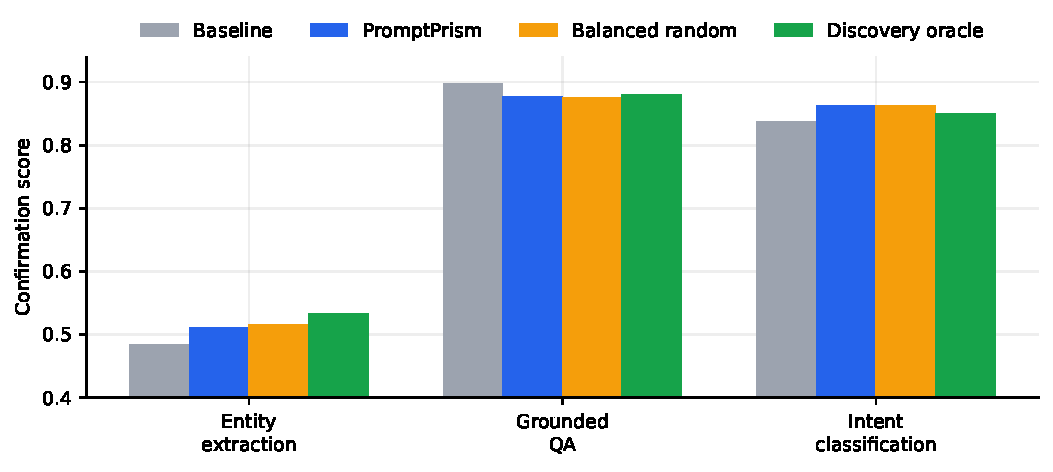
\includegraphics[width=\textwidth]{figures/fig_real_v3_scores.pdf}
\caption{Confirmation scores. ``Oracle'' is selected on discovery and evaluated on confirmation.}
\end{subfigure}\hfill
\begin{subfigure}[b]{0.33\textwidth}
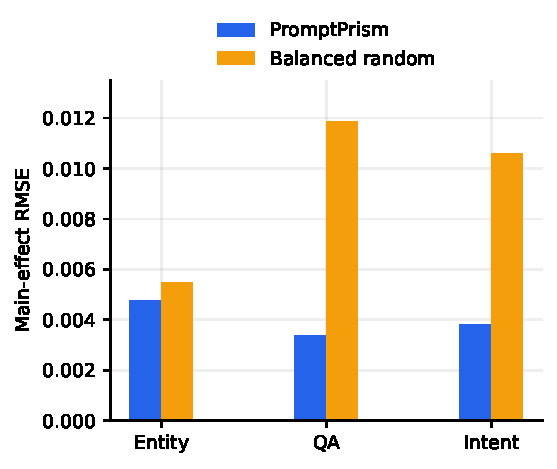
\includegraphics[width=\textwidth]{figures/fig_real_v3_effect_rmse.pdf}
\caption{Main-effect RMSE against the full discovery cube.}
\end{subfigure}
\caption{Registered real-v3 results. Higher scores are better in the left panel; lower RMSE is better in the right panel.}
\label{fig:results}
\end{figure*}

\subsection{Effect recovery, baseline comparison, and uplift}

\begin{table*}[htbp]
\centering
\small
\caption{Effect recovery and discovery-screen resource use. Random RMSE and sign agreement are averaged over twenty frozen balanced designs. Costs use the registered Gemini 2.5 Flash paid-tier rates.}
\label{tab:secondary}
\resizebox{\textwidth}{!}{%
\begin{tabular}{lrrrr}
\toprule
\textbf{Effect recovery} & \textbf{Extraction} & \textbf{QA} & \textbf{Intent} & \textbf{Mean}\\
\midrule
\method\ RMSE & 0.00476 & 0.00339 & 0.00379 & 0.00398\\
Random RMSE & 0.00547 & 0.01188 & 0.01059 & 0.00931\\
\method\ sign agreement & 100.0\% & 83.3\% & 83.3\% & 88.9\%\\
Random sign agreement & 66.7\% & 78.3\% & 77.5\% & 74.2\%\\
\midrule
\textbf{Discovery resources} & \textbf{Configurations} & \textbf{Calls} & \textbf{Total tokens} & \textbf{Cost}\\
\method\ fraction & 16 & 3,840 & 1,138,511 & \$0.5144\\
Mean balanced random screen & 16 & 3,840 & 1,136,752 & \$0.5100\\
Exhaustive cube & 64 & 15,360 & 4,550,470 & \$2.0487\\
\bottomrule
\end{tabular}
}
\end{table*}


The fractional design recovered full-cube marginal effects more accurately than the balanced random screens on every task. Its mean RMSE across tasks was 0.00398, compared with 0.00931 for random screening. Mean sign agreement was 88.9\% versus 74.2\%. This result is descriptive because no separate decision threshold was registered for the across-task effect-recovery summary. It nevertheless distinguishes effect estimation from prompt selection: the fraction can estimate marginal contrasts accurately while its sign-composed recipe fails to beat candidates chosen directly by observed score.

Against run 1, \method\ changed confirmation score by $+0.02769$ for extraction, $-0.02047$ for QA, and $+0.02500$ for intent. None was significant after Benjamini--Hochberg adjustment (adjusted $p=0.4033$, $0.4948$, and $0.4033$, respectively). The fraction of discovery-oracle uplift was 56.2\% for extraction and 200\% for intent; the latter exceeds 100\% because the \method\ recipe generalized better than the discovery-selected oracle. QA was not applicable because the discovery-selected oracle underperformed the baseline on confirmation. These unstable denominators do not support a general uplift claim.

\subsection{Resource use}

The registered fractional discovery screen used 3,840 calls, 1,059,936 input tokens, 78,575 output tokens, and \$0.5144. The exhaustive discovery cube used 15,360 calls, 4,239,744 input tokens, 310,726 output tokens, and \$2.0487. Thus the fraction used exactly 25\% of the configurations and calls, 25\% of input tokens, 25.3\% of output tokens, and 25.1\% of listed cost. A mean balanced random screen had the same call and input-token budget and cost \$0.5100. Fractional screening therefore provides the expected 75\% reduction relative to exhaustive screening, but no resource advantage over its budget-matched primary comparator.

\section{Discussion}

The primary conclusion is direct: in this Gemini 2.5 Flash experiment, a 16-run Resolution IV main-effects screen did not select prompts that generalized better than equal-budget balanced random screening. The estimated difference was very close to zero and its uncertainty spanned both directions. Reporting the negative result matters because orthogonality and effect-estimation precision can otherwise be mistaken for a guarantee of selection performance.

The secondary result explains why fractional designs may still be useful. The fraction estimated the six full-cube marginal contrasts consistently better than random subsets. Teams that need attribution---for example, whether demonstrations or a strict output contract help on average---receive that information with one quarter of the exhaustive configurations. Direct random selection targets a different objective: it can benefit from interactions by choosing a high observed cell without modeling why that cell worked.

The selected recipes also illustrate the limitation of sign composition. \method\ selected runs 28, 16, and 49 for extraction, QA, and intent, while exhaustive discovery selected runs 20, 6, and 50. The selected recipes need not have been observed in the 16-run fraction. A small contrast near zero can flip a component, and multiple sign choices can combine into a configuration affected by interactions. Hierarchical shrinkage, uncertainty-aware factor inclusion, foldover designs, or a final candidate-validation stage are plausible improvements, but they were not tested here.

\paragraph{Limitations.}
The claim is bounded to one requested and returned Gemini model version, one deterministic decoding setup, six particular prompt components, and three tasks. Banking77 was reduced to ten related labels, and the public test/development corpora may have appeared in model training. Only one API execution was made per cell; item resampling quantifies item uncertainty but not repeated generation or model-version drift. The random comparator averages twenty frozen screens, whereas a practitioner normally runs one. The prospective lock was local rather than externally timestamped. Finally, a 95\% interval of roughly $\pm0.028$ is too wide to claim equivalence between the selection procedures.

\section{Reproducibility and artifact trail}

The raw discovery and confirmation manifests, frozen recommendations, locks, summary, CSV results, public source snapshots, split files, and executable analysis are stored under \texttt{research/}. The final manifest SHA-256 hashes are:
\begingroup\scriptsize
\begin{itemize}[leftmargin=*]
\item discovery: \url{2510ed02d94a9e4254fe6911c8f939b4a82248903e84cb57b687ca0617190178};
\item confirmation: \url{88ab4d6d4f1f1f7efb1a3f9d198322df65579085b19090ec3d4ede80b34e7adc};
\item recommendations: \url{cbd5c83c5d95dbfa2b4d1edbff3067450f285e127eb70f1870c8c7aca9be52c6}.
\end{itemize}
\endgroup
The exact protocol describes tie handling, failure scoring, resampling, selection, and the one-sided decision rule. The earlier real-Gemini artifacts remain in their original namespace and are explicitly excluded from this analysis.

\section{Conclusion}

A Resolution IV prompt screen estimated marginal component effects with substantially less error than balanced random subsets and reduced discovery cost by about 75\% relative to exhaustive evaluation. It did not improve held-out prompt selection over balanced random screening: the preregistered primary statistic was $+0.00110$ with $p=0.4568$, in the direction of a negligible random-search advantage. Fractional factorial designs are supported here as efficient tools for structured attribution, while superiority as prompt selectors remains unproven and should be tested across additional models, tasks, and interaction-aware selection rules.

\bibliographystyle{plainnat}
\bibliography{references}
\end{document}
